Testing is an important part of any kind of development, be it software development or other kinds of development.
This section presents the different kinds of tests performed.

\section{Performance} \label{sec:results-performance}

Using performance optimization ideas from \cite{xilinx-speed-strategies}, different synthesization settings were tested and measured to see what gave the best results.
Performance was measured using the maximum frequency estimate output by the XST synthesize process.
Higher maximum frequency is better.

Before optimization, with only default settings, the maximum frequency was given as 42.793Mhz.
When synthesizing with the ``disable dsp usage'' on, the maximum frequency rose to 55.117Mhz, at the cost of a longer runtime for the synthesis process.
Disabling resource sharing when synthesizing further increased the maximum frequency to 56.277Mhz.
Interestingly, increasing the optimization level from ``Normal'' to ``High'' yielded lower results.
All the other settings (all were tested) showed no difference, and they were kept at the default values.

\section{Energy Efficiency}

Because the processor has not been successfully run on an FPGA, it is difficult to perform meaningful energy efficiency testing.
However, ISE provides a ``Generate Power Data'' process, which can be used to assess ballpark measurements.
Table \vref{table:power-data} shows generated power data.
The synthesis process offers a setting called ``Power Reduction''.
This setting has no effect on the generated power data.

\begin{table}

\begin{center}
\begin{tabular}{ | l | r | r | r | r | }
\hline
\multicolumn{5}{ | c | }{On-Chip Power Summary} \\
\hline
On-Chip & Power (mW) & Used & Available & Utilization (\%) \\
\hline
Clocks & 0.04 & 1 & --- & --- \\
Logic & 0.00 & 3134 & 9112 & 34 \\
Signals & 0.00 & 3762 & --- & --- \\
IOs & 0.00 & 138 & 232 & 59 \\
BlockRAM/FIFO & 0.00 & --- & --- & --- \\
- 8K BlockRAM & 0.00 & 2 & 64 & 3 \\
- 16K BlockRAM & 0.00 & 0 & 32 & 0 \\
Quiescent & 14.84 & & & \\
Total & 14.89 & & & \\
\hline
\end{tabular}

\bigskip

\begin{tabular}{| l | l | l | l |}
\hline
\multicolumn{4}{ | c |}{Power Supply Summary} \\
\hline
 & Total & Dynamic & Quiescent \\
\hline
Supply Power (mW) & 14.89 & 0.04 & 14.84 \\
\hline
\end{tabular}

\bigskip

\begin{tabular}{ | l | r | r | r | r |}
\hline
\multicolumn{5}{ | c | }{Power Supply Currents} \\
\hline
\multicolumn{1}{ | c | }{Supply Source} & Supply Voltage & Total Current (mA) & Dynamic Current (mA) & Quiescent Current (mA) \\
\hline
Vccint & 1.200 & 6.12 & 0.04 & 6.08 \\
Vccaux & 2.500 & 3.02 & 0.00 & 3.02 \\
Vcco25 & 2.500 & 0.00 & 0.00 & 0.00 \\
\hline
\end{tabular}

\caption{Generated Power Data}
\label{table:power-data}
\end{center}
\end{table}

\section{VHDL Test Benches}

In VHDL, one has the opportunity to create test benches to validate VHDL components.
A test bench is a piece of VHDL code that instantiates a component, manipulates its in-signals, and measures the resulting output the component sends out again.
It is the hardware design analog of unit testing in regular software development.
These test benches are typically run in simulator software such as ISim or ModelSim, which simulates hardware in an easily measurable and inspectable environment.

Generally, each component made in VHDL should have a corresponding test bench.
Because a component is typically defined in its own file, a common test bench scheme is to have one file, ``\texttt{my\_entity.vhd}'', which defines the component, and one file, ``\texttt{tb\_my\_entity.vhd}'', which defines the test bench for the component.
Of course, here \texttt{my\_component} is a placeholder name for a component.

In this assignment, each component has an corresponding automatic test bench, which aims to verify correct functionality for a component.
The tests were run in the hardware simulation tool called ISim 12.4 (nt64).

\subsection{ALU Test Bench}

The ALU is continuously receiving values for X, Y and Func, and will use this input to set the correct values for R and the flags.
The test bench include tests for the outputs for each of the ALUs supported functions.
In addition the subtraction function is tested extra thoroughly.
This is because of its involvement in the branch operations.

Figure \vref{figure:tb-alu} is a screen capture of the test bench running in ModelSim.

\subsection{Branch Controller Test Bench}

The branch controller is a logical unit that will continuously determine if the ALU should compare to a zero value and whether or not to branch.
The test will check each branching operation and test that the compare\_zero and compare\_zero\_value have the correct values.
The test will also check each of these operations with their sensitive flag on and off, and test that branch have the right value.
For good measure we also check that all values are set \texttt{to} 0 when the operation is not a branching operation.
This last test is not really necessary in the current processor layout as the branching MUX will remove the signal eventually.

Figure \vref{figure:tb-branch-controller} is a screen capture of the test bench running in ModelSim.

\subsection{MUX Test Bench}

The MUX is really quite simple, and so is its test.
The test puts two different signals on the input ports and reads each of these through each of the input ports.

Figure \vref{figure:tb-mux} is a screen capture of the test bench running in ModelSim.

\subsection{PC Test Bench}

The program counter have several inputs which on each rising edge on the clock will reevaluate what value to put out of the program counter.
There are several ways the program counter can act:
\begin{itemize}
\item{If reset is set to \texttt{1}, it will reset pc\_out to \texttt{0}.}
\item{If both pc enable and reset is set to \texttt{1}, it should still reset.}
\item{If pc enable is set to \texttt{0}, it will not load a new value from pc\_in.}
\item{If pc enable is set to \texttt{1}, pc\_out will be set to the value of pc\_in.}
\end{itemize}
The pc test bench confirms that each of these four behaviors work as intended.

Figure \vref{figure:tb-pc} is a screen capture of the test bench running in ModelSim.


\subsection{Processor Test Bench}

The processor test bench tests that the processor acts as expected on a few operations.
First it loads some words into registers.
When the data is ready, the test performs some arithmetical and logical operations on the data.
In the end the data is written back to memory.
The purpose of this test is not to cover all the operations, as they are already covered in the ALU test bench, but rather test each class of operation to verify that they work.
The processor test bench makes sure that all the processor components work together as intended, and that the processor is able to execute memory load and store operations.
Figure \vref{figure:tb-processor} is a screen capture of the test bench running in ModelSim.

\subsection{Toplevel Test Bench}

The toplevel test bench defines a short program of 16 binary-coded instructions that it uses to test the processor.
These instructions are helpfully named \texttt{ins0} through \texttt{ins15}.
A comment in the the test bench refers to a certain \texttt{ins.txt}, which supposedly contains a description of the instructions, but it is nowhere to be found.
A manually decoded program listing of this program can be found in listing \vref{listing:toplevel-program}.

\begin{listing}
\begin{center}
\begin{bytefield}[rightcurly=., rightcurlyspace=0pt, leftcurly=., leftcurlyspace=0pt]{32}
\bitheader[endianness=big]{0-16,20,21,25,26,31} \\

\begin{rightwordgroup}{\texttt{lw r0, 1(r0)}}
\begin{leftwordgroup}{\texttt{ins0}}
\bitbox{6}{op: lw \\ \tiny 100011}
& \bitbox{5}{rs: r0 \\ \tiny 00000}
& \bitbox{5}{rt: r1 \\ \tiny 00001}
& \bitbox{16}{immediate: 1 \\ \tiny 0000000000000001}
\end{leftwordgroup}
\end{rightwordgroup} \\

\begin{rightwordgroup}{\texttt{lw r2, 2(r0)}}
\begin{leftwordgroup}{\texttt{ins1}}
\bitbox{6}{op: lw \\ \tiny 100011}
& \bitbox{5}{rs: r0 \\ \tiny 00000}
& \bitbox{5}{rt: r2 \\ \tiny 00010}
& \bitbox{16}{immediate: 1 \\ \tiny 0000000000000010}
\end{leftwordgroup}
\end{rightwordgroup} \\

\begin{rightwordgroup}{\texttt{lw r2, 2(r0)}}
\begin{leftwordgroup}{\texttt{ins2}}
\bitbox{6}{op: lw \\ \tiny 100011}
& \bitbox{5}{rs: r0 \\ \tiny 00000}
& \bitbox{5}{rt: r2 \\ \tiny 00010}
& \bitbox{16}{immediate: 1 \\ \tiny 0000000000000010}
\end{leftwordgroup}
\end{rightwordgroup} \\

\begin{rightwordgroup}{\texttt{add r3, r1, r2}}
\begin{leftwordgroup}{\texttt{ins3}}
\bitbox{6}{op: r\_all \\ \tiny 000000}
& \bitbox{5}{rs: r1 \\ \tiny 00001}
& \bitbox{5}{rt: r2 \\ \tiny 00010}
& \bitbox{5}{rd: r3 \\ \tiny 00011}
& \bitbox{5}{sh: 0 \\ \tiny 00000}
& \bitbox{6}{func: add \\ \tiny 100000}
\end{leftwordgroup}
\end{rightwordgroup} \\

\begin{rightwordgroup}{\texttt{sw r3, 5(r0)}}
\begin{leftwordgroup}{\texttt{ins4}}
\bitbox{6}{op: sw \\ \tiny 101011}
& \bitbox{5}{rs: r0 \\ \tiny 00000}
& \bitbox{5}{rt: r3 \\ \tiny 00011}
& \bitbox{16}{imm: 5 \\ \tiny 0000000000000101}
\end{leftwordgroup}
\end{rightwordgroup} \\

\begin{rightwordgroup}{\texttt{beq r0, r0, 5}}
\begin{leftwordgroup}{\texttt{ins5}}
\bitbox{6}{op: beq \\ \tiny 000100}
& \bitbox{5}{rs: r0 \\ \tiny 00000}
& \bitbox{5}{rt: r0 \\ \tiny 00000}
& \bitbox{16}{imm: 5 \\ \tiny 0000000000000101}
\end{leftwordgroup}
\end{rightwordgroup} \\

\begin{rightwordgroup}{\texttt{sw r3, 3(r0)}}
\begin{leftwordgroup}{\texttt{ins6}}
\bitbox{6}{op: sw \\ \tiny 101011}
& \bitbox{5}{rs: r0 \\ \tiny 00000}
& \bitbox{5}{rt: r3 \\ \tiny 00011}
& \bitbox{16}{imm: 3 \\ \tiny 0000000000000011}
\end{leftwordgroup}
\end{rightwordgroup} \\

\begin{rightwordgroup}{\texttt{sw r3, 4(r0)}}
\begin{leftwordgroup}{\texttt{ins7}}
\bitbox{6}{op: sw \\ \tiny 101011}
& \bitbox{5}{rs: r0 \\ \tiny 00000}
& \bitbox{5}{rt: r3 \\ \tiny 00011}
& \bitbox{16}{imm: 4 \\ \tiny 0000000000000100}
\end{leftwordgroup}
\end{rightwordgroup} \\

\begin{rightwordgroup}{\texttt{sw r3, 6(r0)}}
\begin{leftwordgroup}{\texttt{ins8}}
\bitbox{6}{op: sw \\ \tiny 101011}
& \bitbox{5}{rs: r0 \\ \tiny 00000}
& \bitbox{5}{rt: r3 \\ \tiny 00011}
& \bitbox{16}{imm: 6 \\ \tiny 0000000000000110}
\end{leftwordgroup}
\end{rightwordgroup} \\

\begin{rightwordgroup}{\texttt{sw r3, 7(r0)}}
\begin{leftwordgroup}{\texttt{ins9}}
\bitbox{6}{op: sw \\ \tiny 101011}
& \bitbox{5}{rs: r0 \\ \tiny 00000}
& \bitbox{5}{rt: r3 \\ \tiny 00011}
& \bitbox{16}{imm: 7 \\ \tiny 0000000000000111}
\end{leftwordgroup}
\end{rightwordgroup} \\

\begin{rightwordgroup}{\texttt{lui r3, 6(r0)}}
\begin{leftwordgroup}{\texttt{ins10}}
\bitbox{6}{op: lui \\ \tiny 001111}
& \bitbox{5}{rs: r0 \\ \tiny 00000}
& \bitbox{5}{rt: r3 \\ \tiny 00011}
& \bitbox{16}{imm: 6 \\ \tiny 0000000000000110}
\end{leftwordgroup}
\end{rightwordgroup} \\

\begin{rightwordgroup}{\texttt{sw r3, 8(r0)}}
\begin{leftwordgroup}{\texttt{ins11}}
\bitbox{6}{op: sw \\ \tiny 101011}
& \bitbox{5}{rs: r0 \\ \tiny 00000}
& \bitbox{5}{rt: r3 \\ \tiny 00011}
& \bitbox{16}{imm: 8 \\ \tiny 0000000000001000}
\end{leftwordgroup}
\end{rightwordgroup} \\

\begin{rightwordgroup}{\texttt{add r1, r3, r3}}
\begin{leftwordgroup}{\texttt{ins12}}
\bitbox{6}{op: r\_all \\ \tiny 000000}
& \bitbox{5}{rs: r1 \\ \tiny 00001}
& \bitbox{5}{rt: r3 \\ \tiny 00011}
& \bitbox{5}{rd: r3 \\ \tiny 00011}
& \bitbox{5}{sh: 0 \\ \tiny 00000}
& \bitbox{6}{func: add \\ \tiny 100000}
\end{leftwordgroup}
\end{rightwordgroup} \\

\begin{rightwordgroup}{\texttt{sw r3, 9(r0)}}
\begin{leftwordgroup}{\texttt{ins13}}
\bitbox{6}{op: sw \\ \tiny 101011}
& \bitbox{5}{rs: r0 \\ \tiny 00000}
& \bitbox{5}{rt: r3 \\ \tiny 00011}
& \bitbox{16}{imm: 9 \\ \tiny 0000000000001001}
\end{leftwordgroup}
\end{rightwordgroup} \\

\begin{rightwordgroup}{\texttt{beq r0, r0, -3}}
\begin{leftwordgroup}{\texttt{ins14}}
\bitbox{6}{op: beq \\ \tiny 000100}
& \bitbox{5}{rs: r0 \\ \tiny 00000}
& \bitbox{5}{rt: r0 \\ \tiny 00000}
& \bitbox{16}{imm: -3 \\ \tiny 1111111111111101}
\end{leftwordgroup}
\end{rightwordgroup} \\

\begin{rightwordgroup}{\texttt{sw r3, 10(r0)}}
\begin{leftwordgroup}{\texttt{ins15}}
\bitbox{6}{op: sw \\ \tiny 101011}
& \bitbox{5}{rs: r0 \\ \tiny 00000}
& \bitbox{5}{rt: r3 \\ \tiny 00011}
& \bitbox{16}{imm: 10 \\ \tiny 0000000000001010}
\end{leftwordgroup}
\end{rightwordgroup} \\

\end{bytefield}
\end{center}
\caption{The short program in the toplevel test bench}
\label{listing:toplevel-program}
\end{listing}


Figure \vref{figure:tb-toplevel} is a screen capture of the test bench running in ModelSim.

\section{Testing on the Spartan-6 FPGA}

It is also possible to run tests directly on the FPGA.
This was unfortunately not done, as the processor was never successfully loaded onto the FPGA.


\begin{figure}
	\begin{center}
		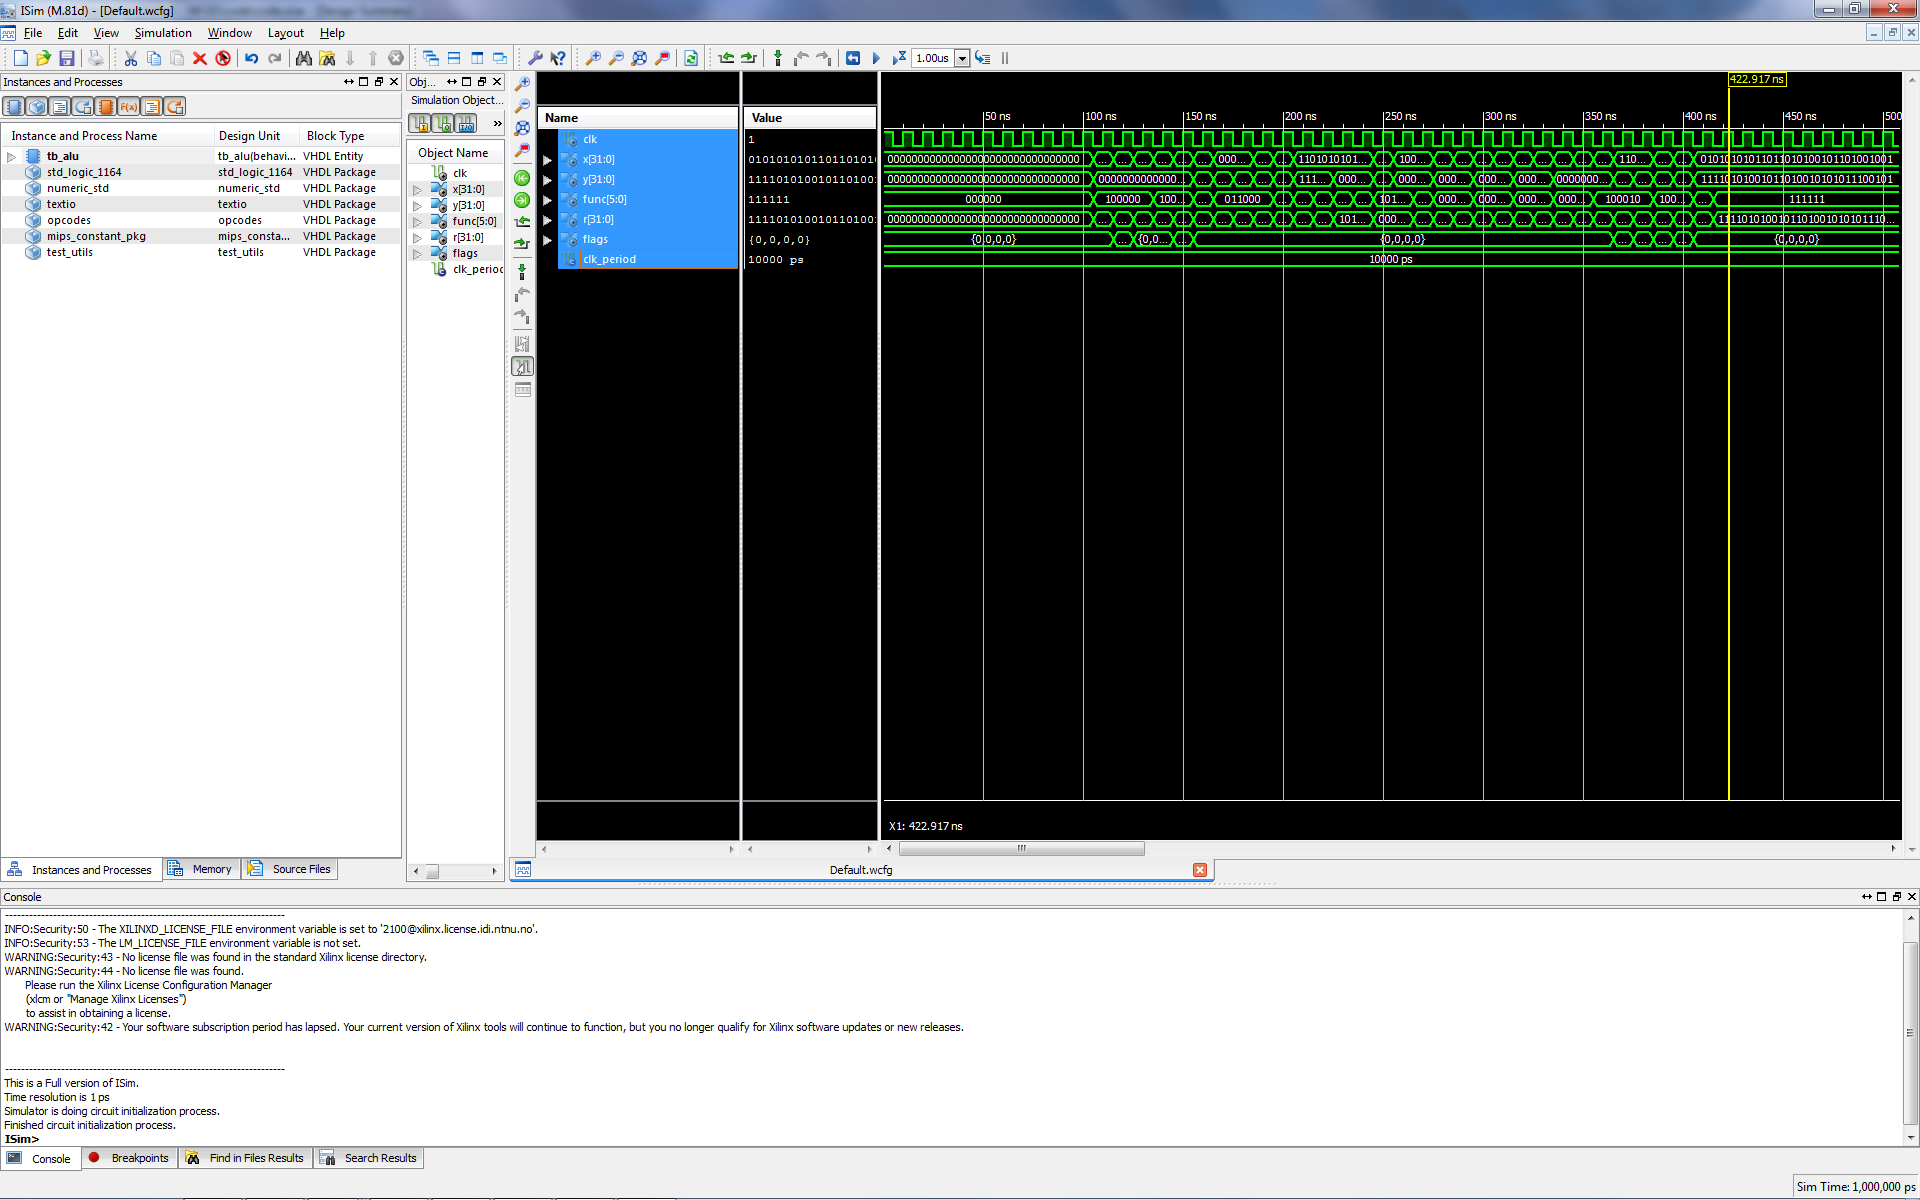
\includegraphics[keepaspectratio, width=\textwidth]{graphics/tb_alu.PNG}
		\caption{Screen capture of the ALU test bench running in ModelSim}
		\label{figure:tb-alu}
	\end{center}
\end{figure}

\begin{figure}
	\begin{center}
		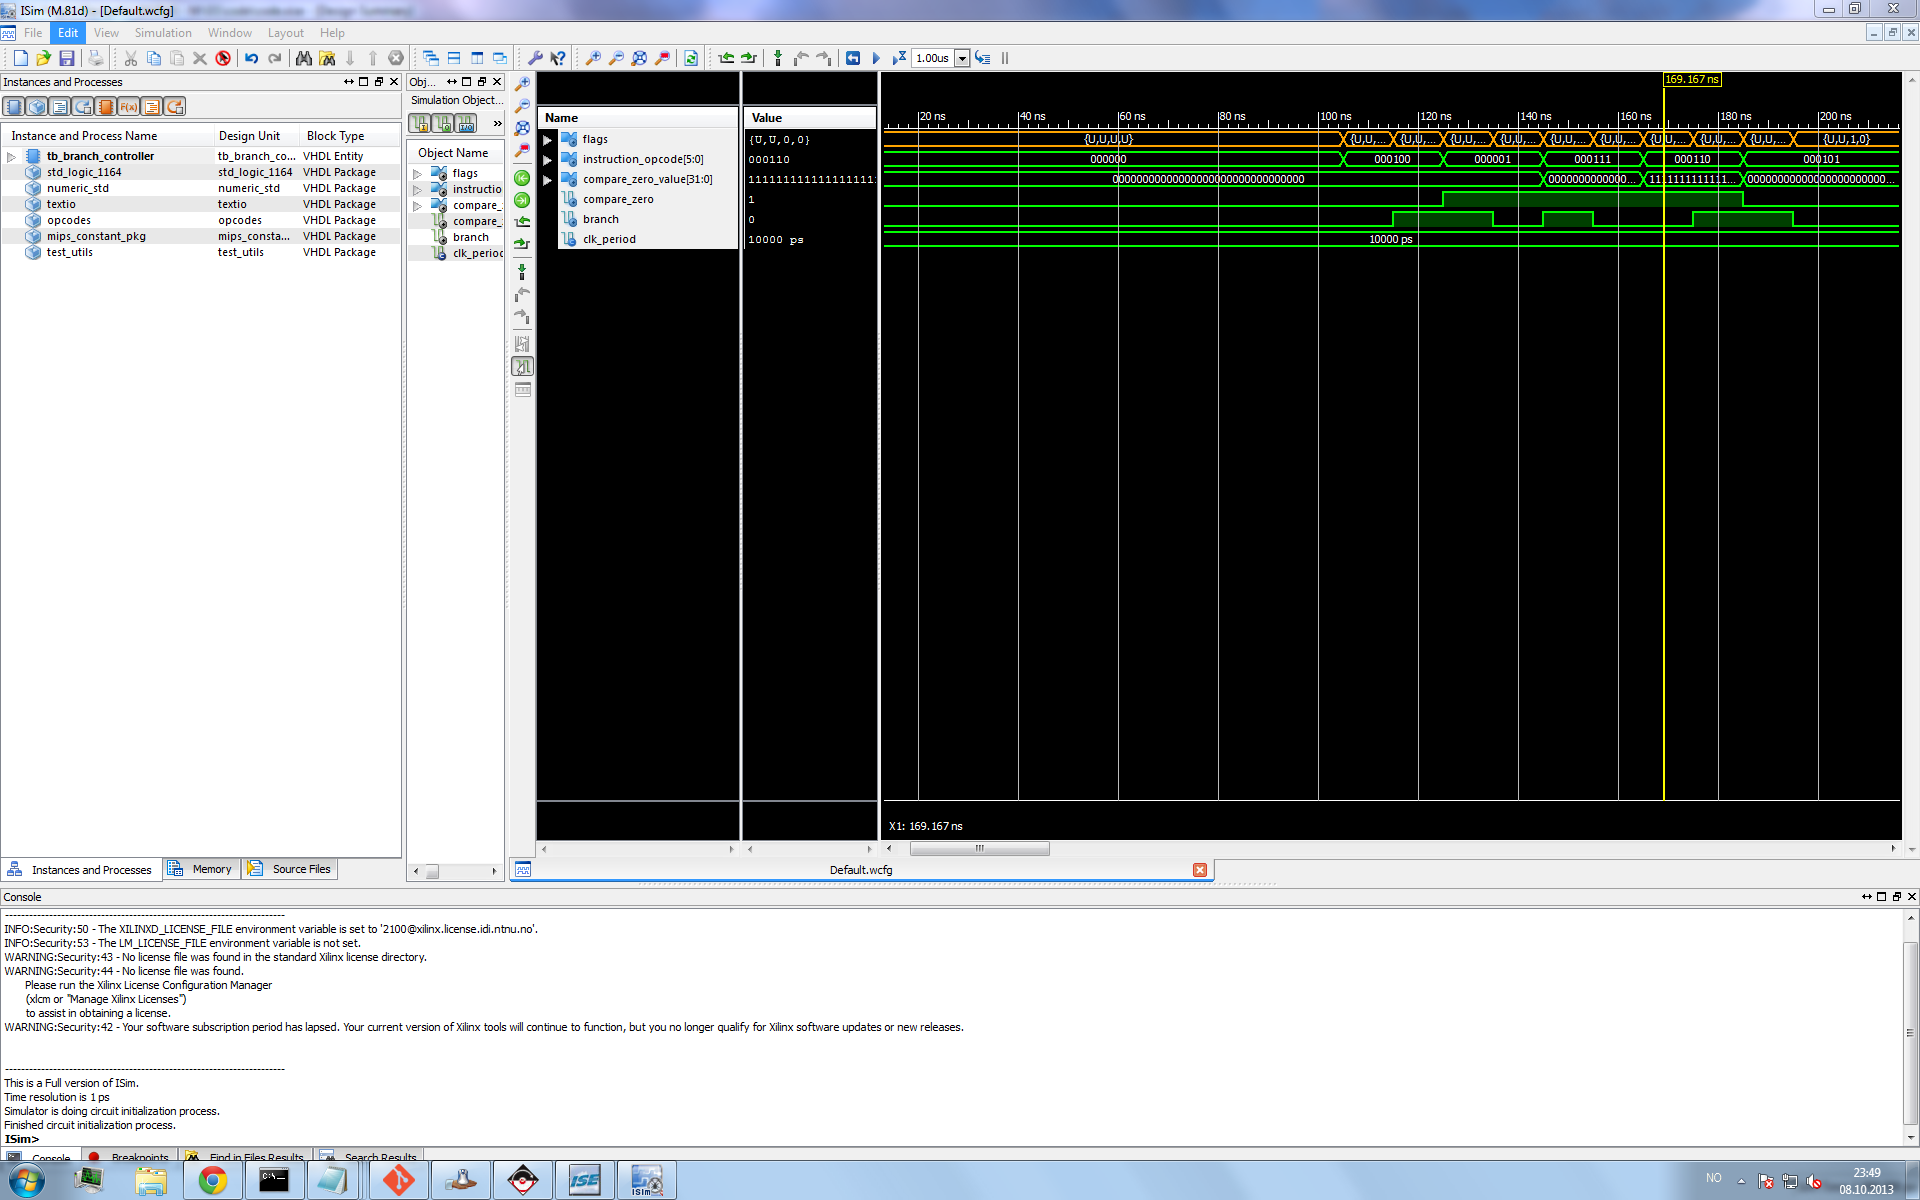
\includegraphics[keepaspectratio, width=\textwidth]{graphics/tb_branch_controller.PNG}
		\caption{Screen capture of the branch controller test bench running in ModelSim}
		\label{figure:tb-branch-controller}
	\end{center}
\end{figure}

\begin{figure}
	\begin{center}
		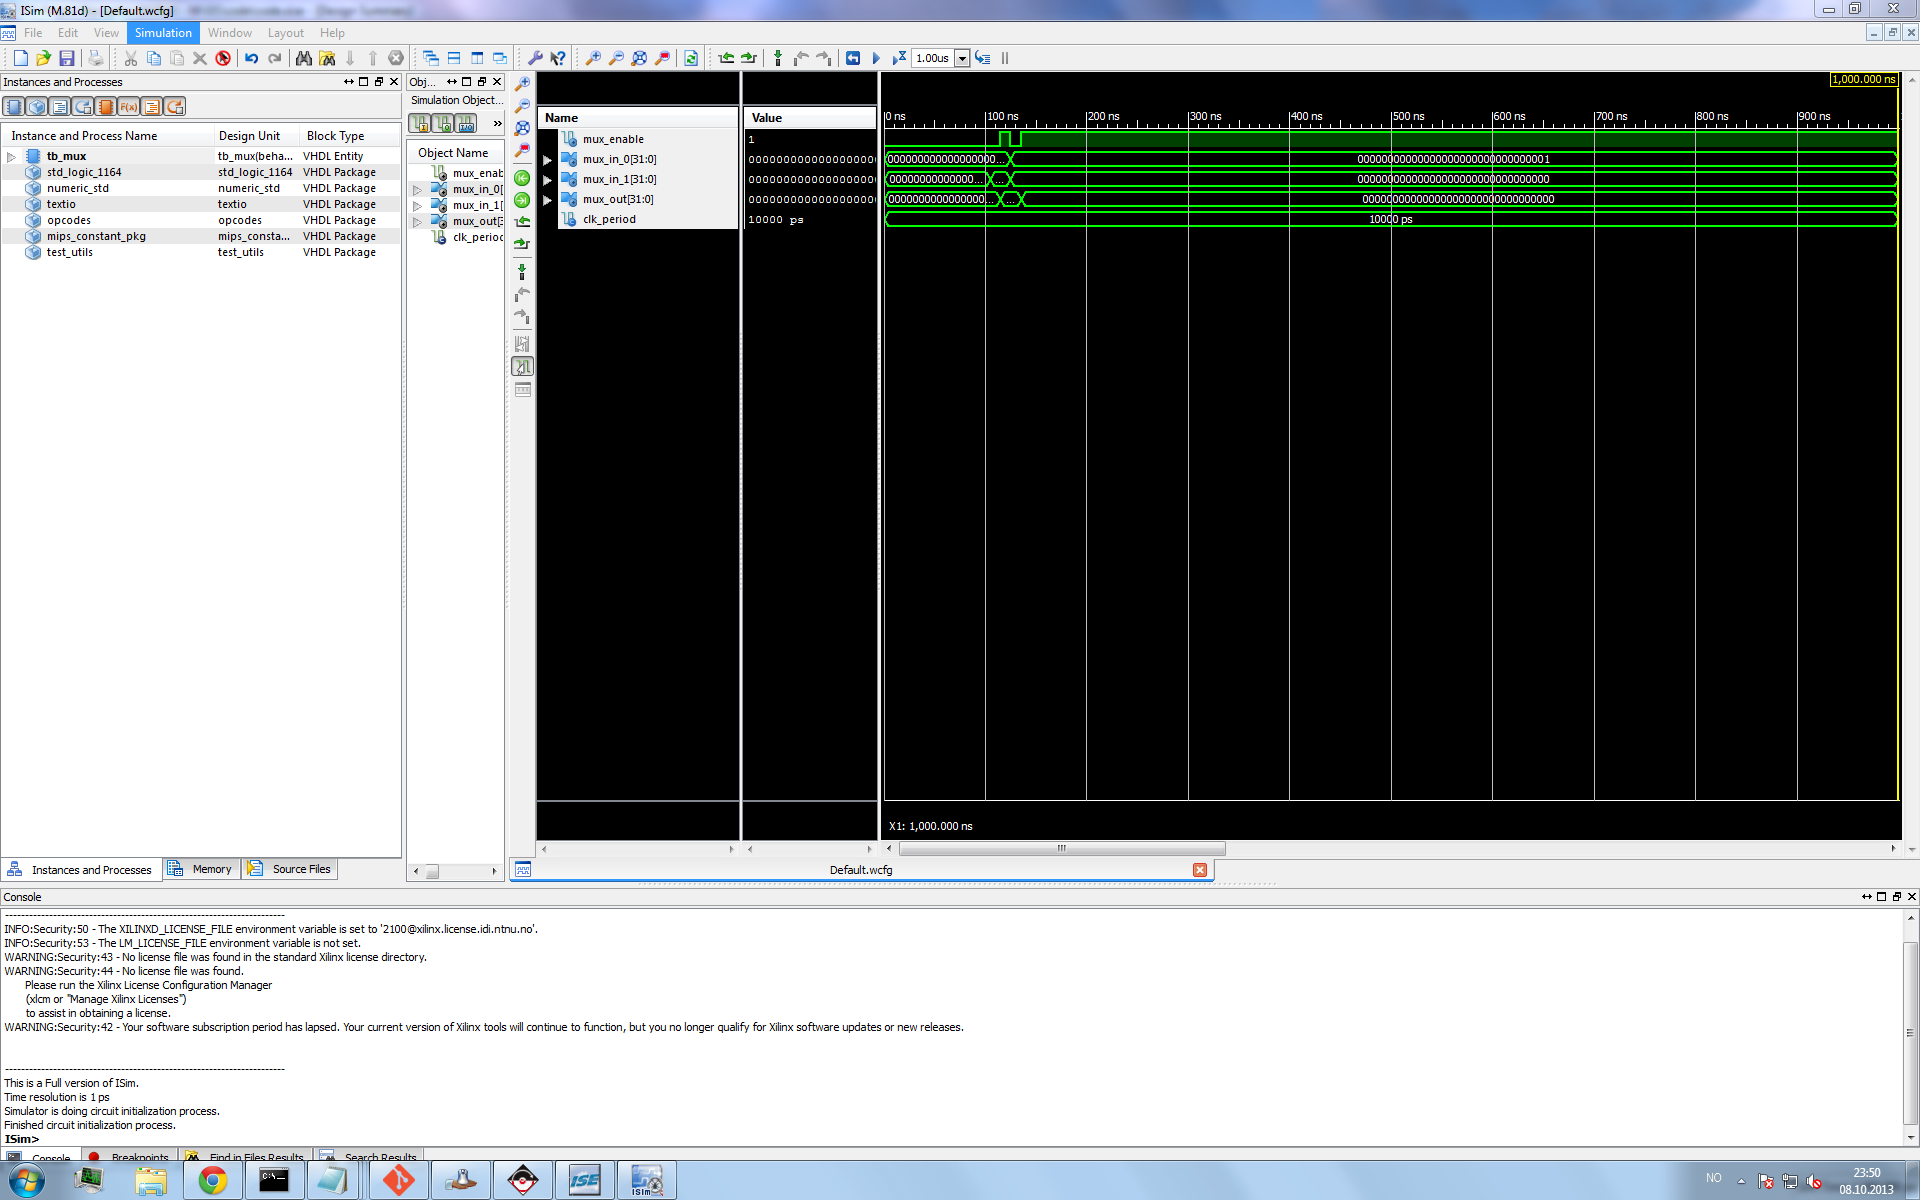
\includegraphics[keepaspectratio, width=\textwidth]{graphics/tb_mux.PNG}
		\caption{Screen capture of the MUX test bench running in ModelSim}
		\label{figure:tb-mux}
	\end{center}
\end{figure}

\begin{figure}
	\begin{center}
		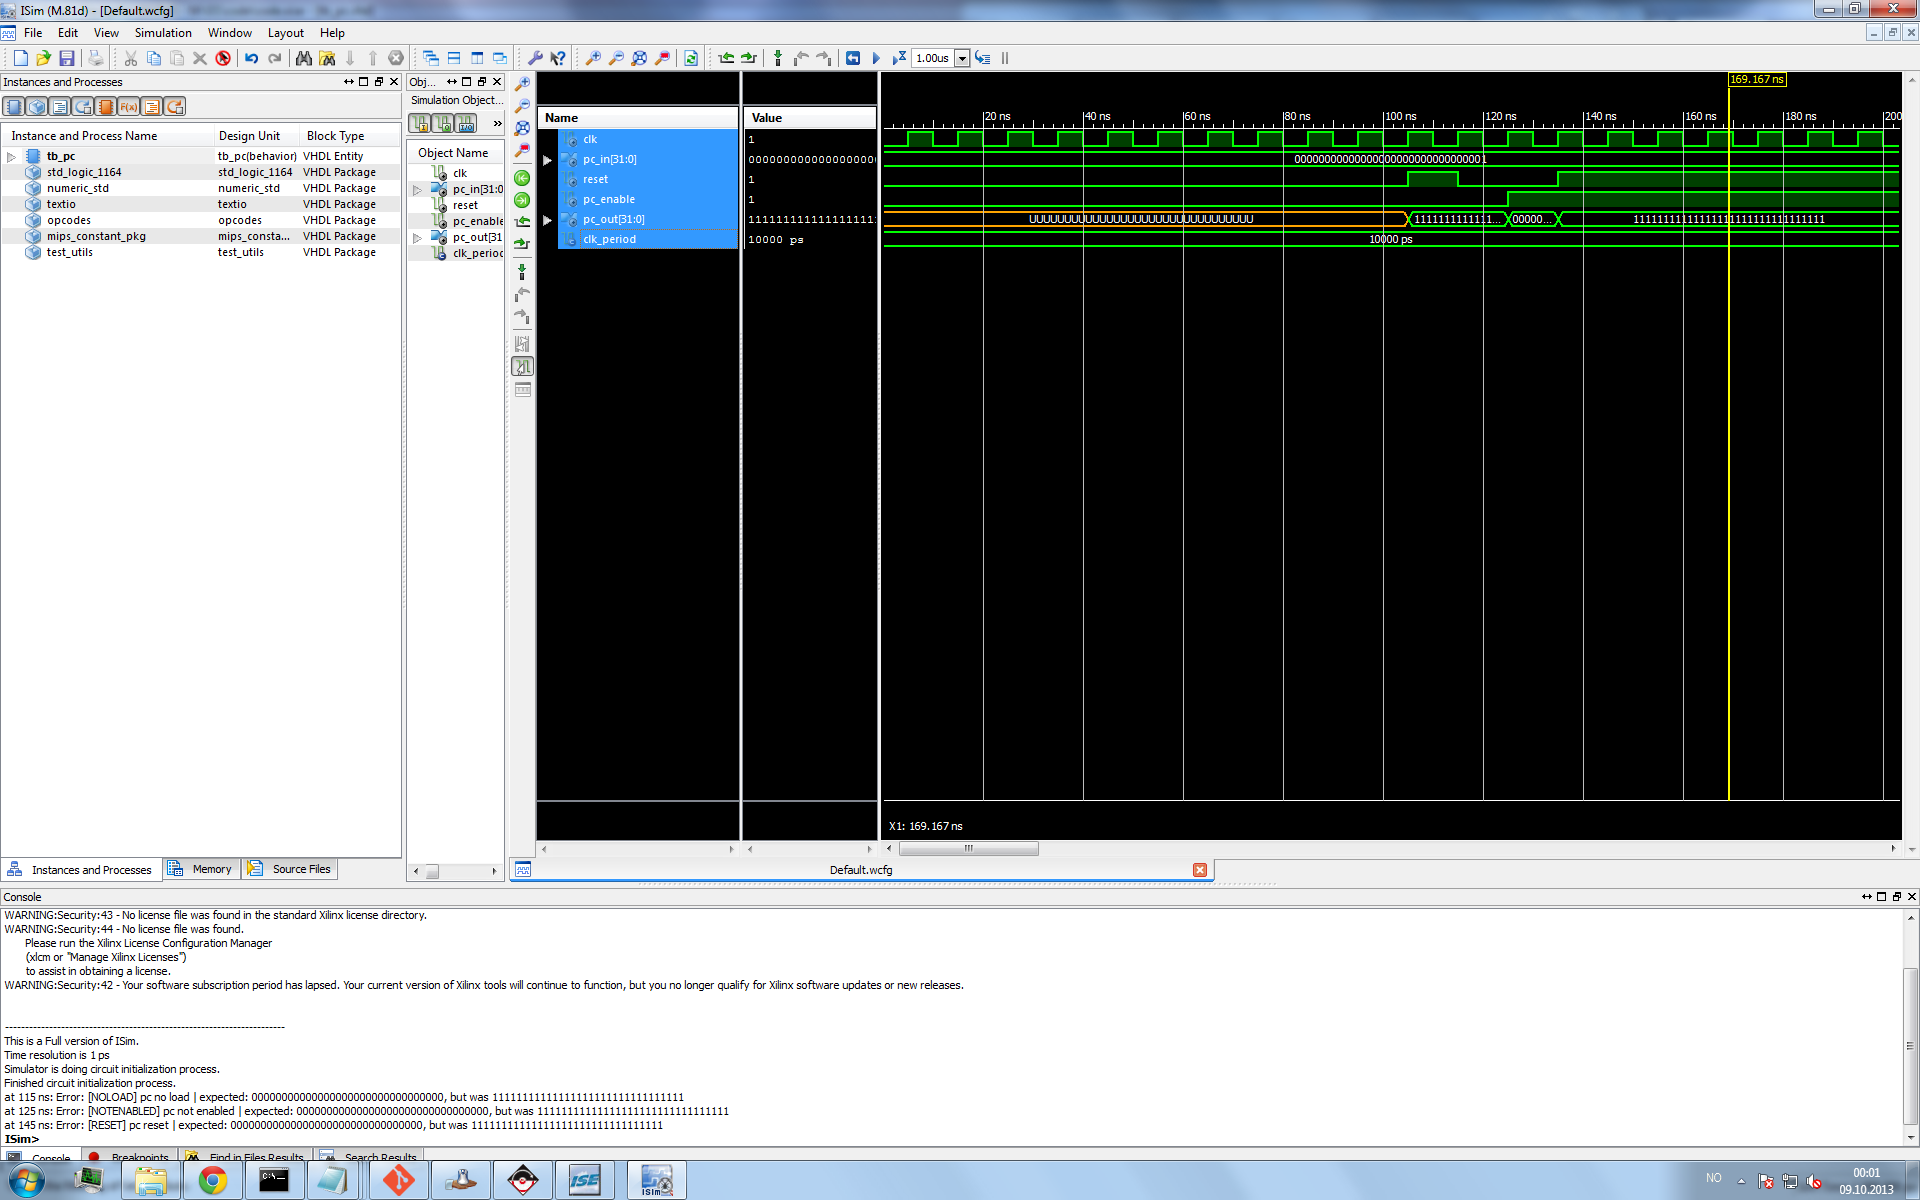
\includegraphics[keepaspectratio, width=\textwidth]{graphics/tb_pc.PNG}
		\caption{Screen capture of the PC test bench running in ModelSim}
		\label{figure:tb-pc}
	\end{center}
\end{figure}

\begin{figure}
	\begin{center}
		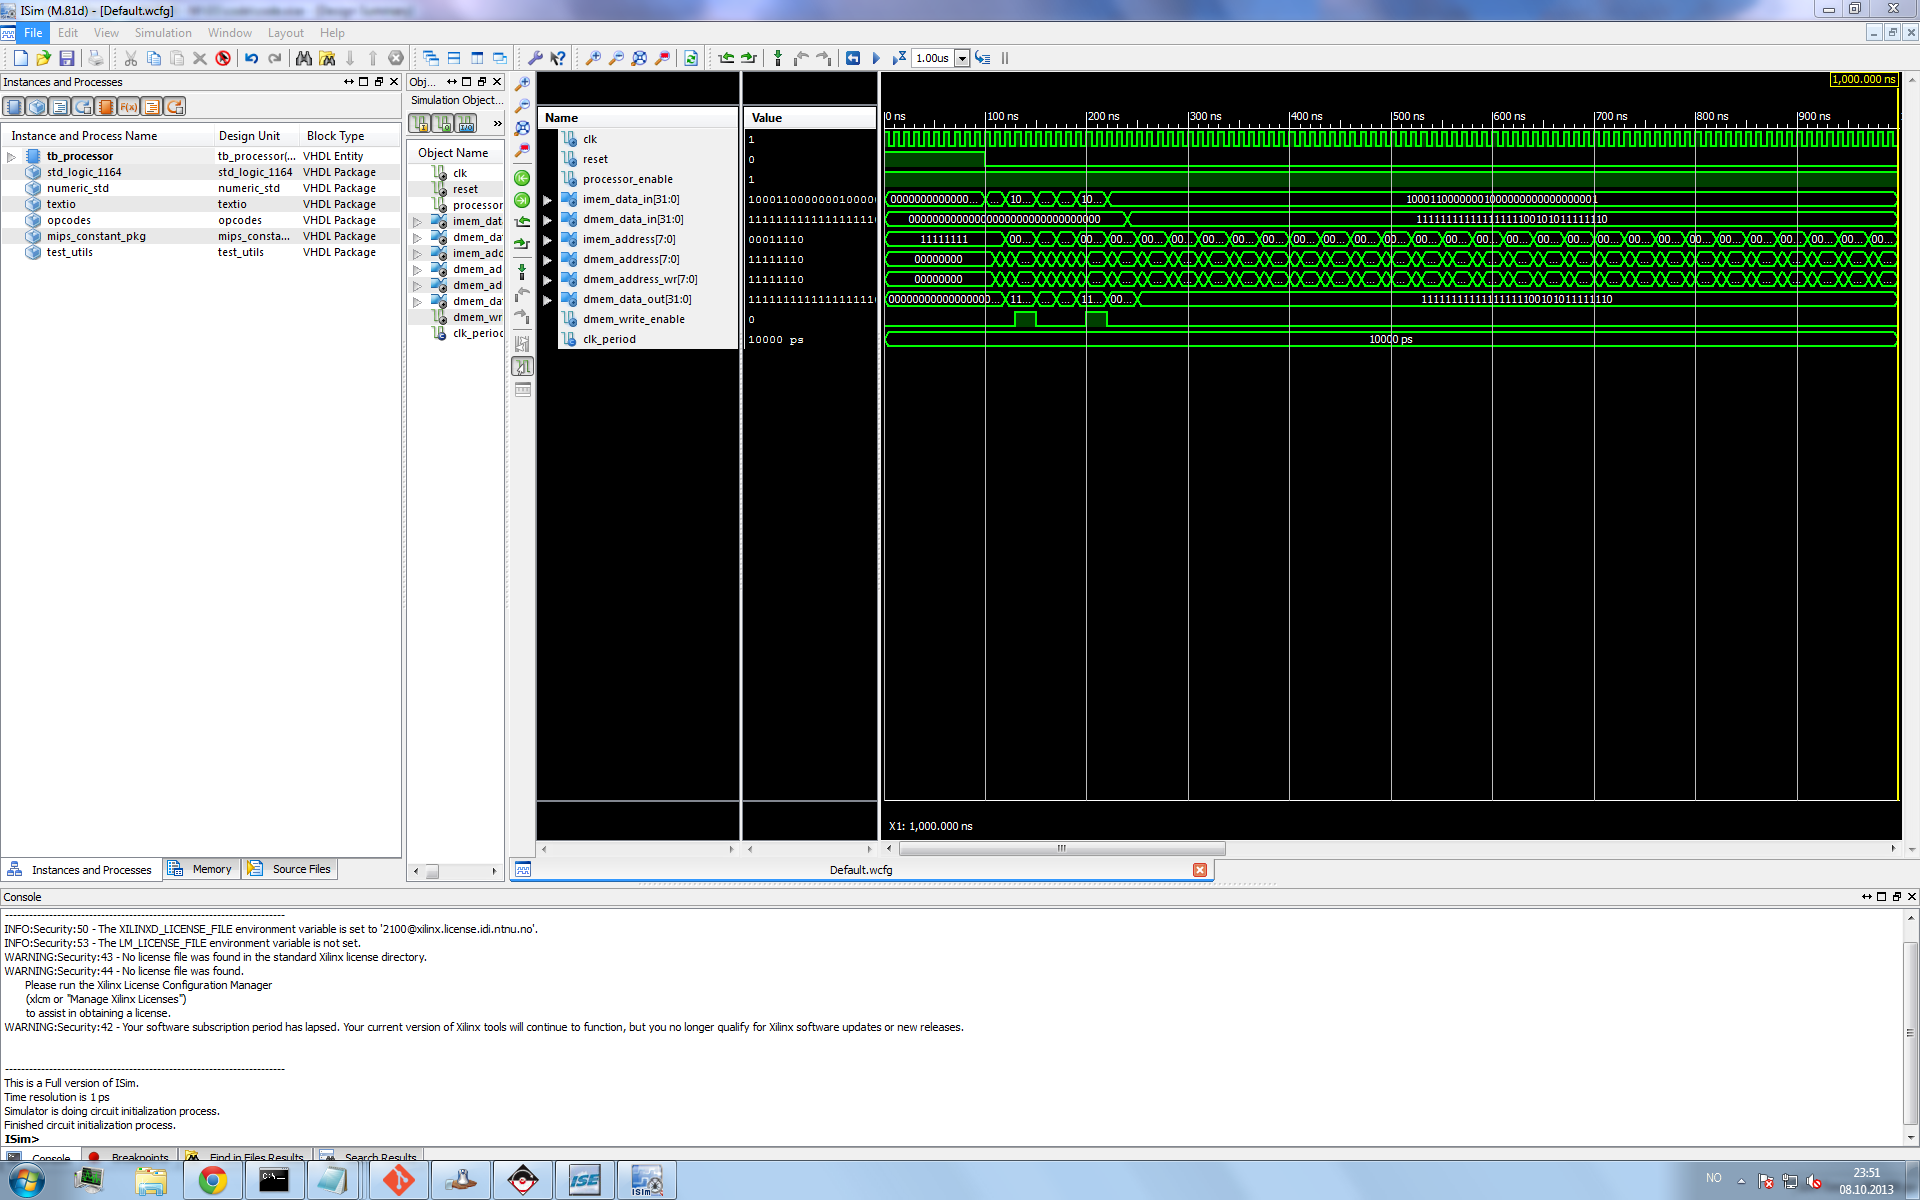
\includegraphics[keepaspectratio, width=\textwidth]{graphics/tb_processor.PNG}
		\caption{Screen capture of the processor test bench running in ModelSim}
		\label{figure:tb-processor}
	\end{center}
\end{figure}

\begin{figure}
	\begin{center}
		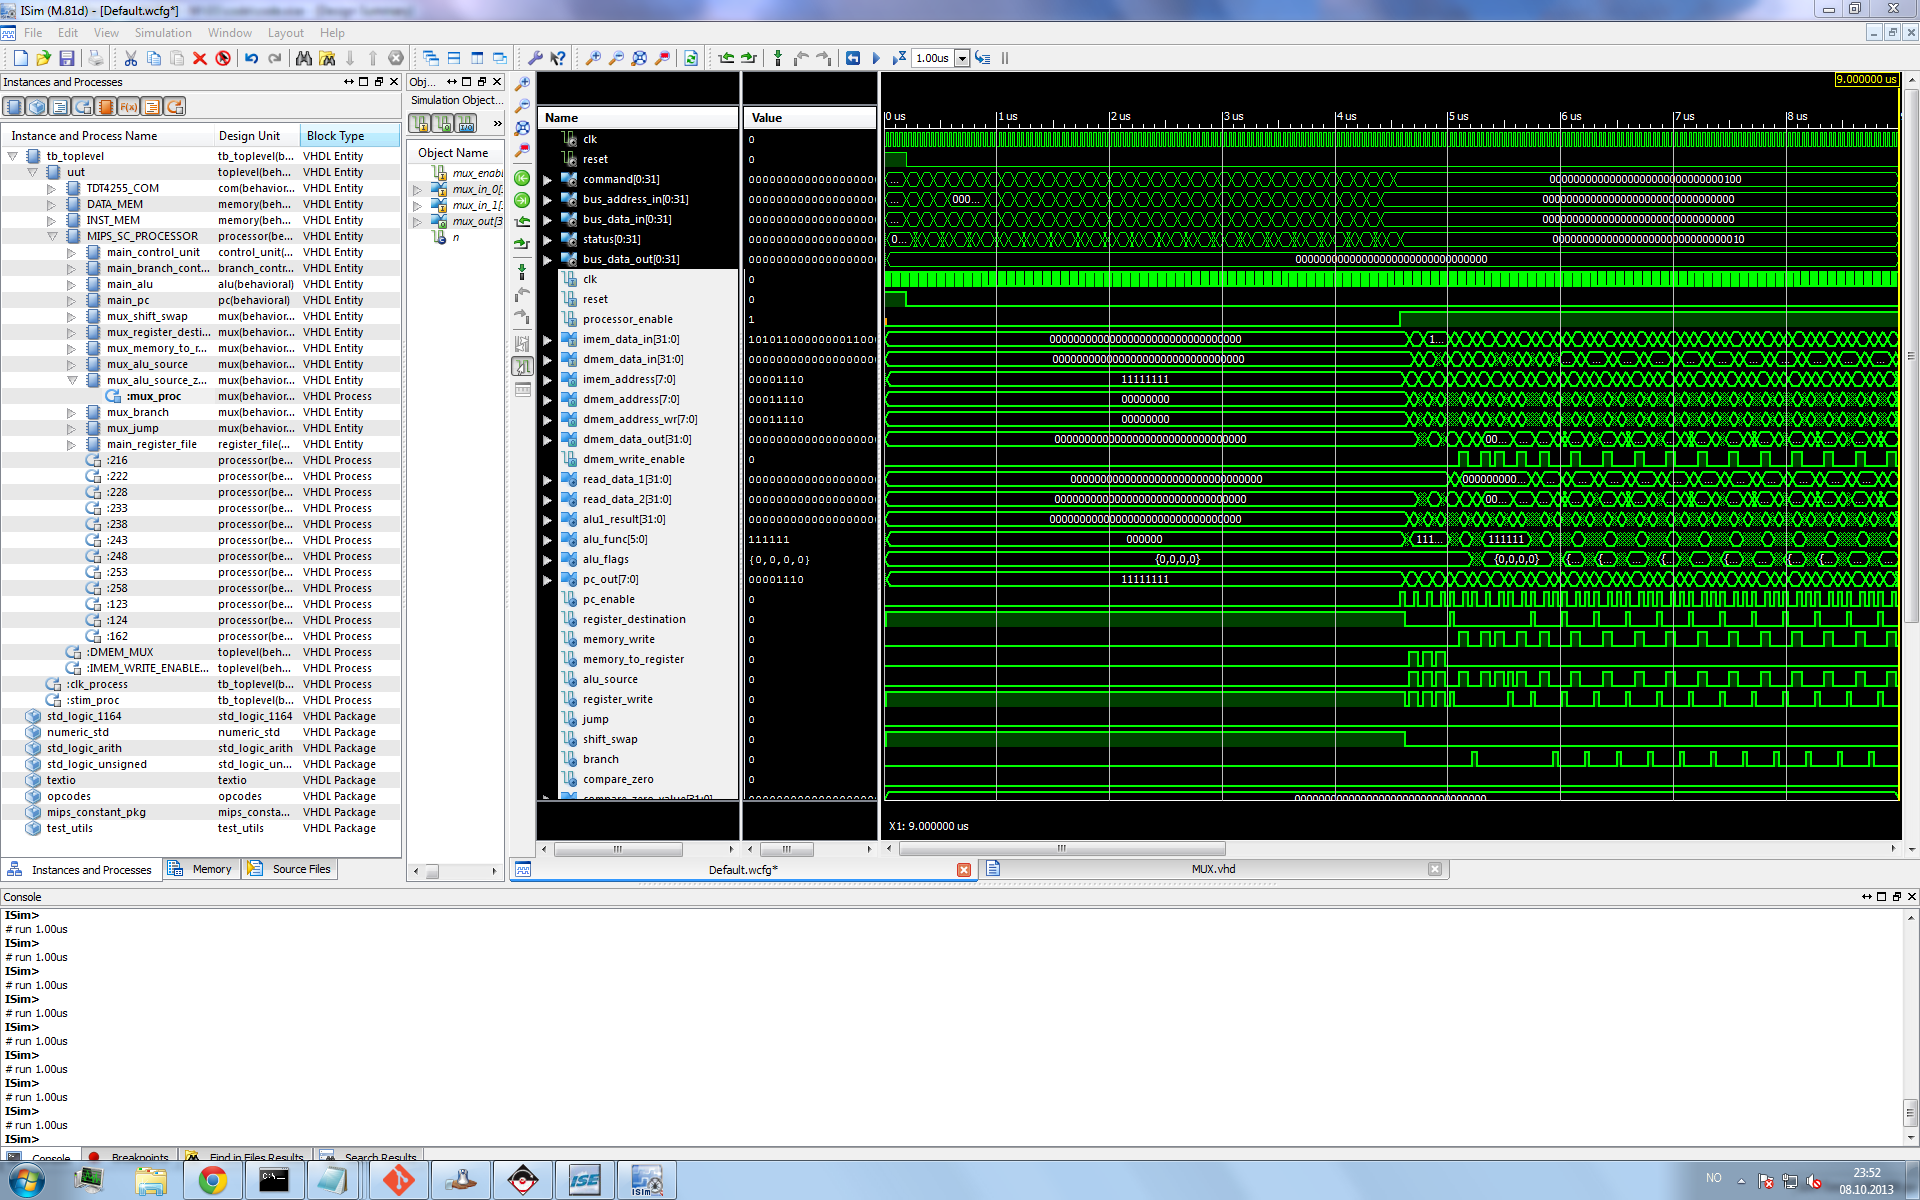
\includegraphics[keepaspectratio, width=\textwidth]{graphics/tb_toplevel.PNG}
		\caption{Screen capture of the toplevel test bench running in ModelSim}
		\label{figure:tb-toplevel}
	\end{center}
\end{figure}
